\documentclass[a4paper,14pt,russian]{extreport} \usepackage{extsizes}
\usepackage{cmap} 
\usepackage[T2A]{fontenc}
\usepackage[utf8]{inputenc}
\usepackage[russian]{babel}
\usepackage{pscyr}
\usepackage{graphicx}  \usepackage{amssymb,amsfonts,amsmath,amsthm}  \usepackage{indentfirst} \usepackage[usenames,dvipsnames]{color}
\usepackage{makecell}
\usepackage{multirow}
\usepackage{ulem} 
\linespread{1.3} 
\renewcommand{\rmdefault}{ftm}
\frenchspacing
\usepackage{fancyhdr}
\pagestyle{fancy}
\fancyhf{}
\fancyhead[R]{\thepage}
\fancyheadoffset{0mm}
\fancyfootoffset{0mm}
\setlength{\headheight}{17pt} \renewcommand{\headrulewidth}{0pt} \renewcommand{\footrulewidth}{0pt} \fancypagestyle{plain}{\fancyhf{} \rhead{\thepage}}
\setcounter{page}{2} % начать нумерацию страниц с №2
\usepackage[tableposition=top]{caption}
\usepackage{subcaption}
\DeclareCaptionLabelFormat{gostfigure}{Рисунок #2} \DeclareCaptionLabelFormat{gosttable}{Таблица #2} \DeclareCaptionLabelSeparator{gost}{~---~}
\captionsetup{labelsep=gost} 
\captionsetup[figure]{labelformat=gostfigure}
\captionsetup[table]{labelformat=gosttable} \renewcommand{\thesubfigure}{\asbuk{subfigure}}
\usepackage{titlesec} 
\titleformat{\chapter}[display]
{\filcenter}
{\MakeUppercase{\chaptertitlename} \thechapter}     {8pt}    
{\bfseries}{} 
\titleformat{\section}
{\normalsize\bfseries}
{\thesection}{1em}{}
\titleformat{\subsection}     
{\normalsize\bfseries}
{\thesubsection}     
{1em}{}
\titlespacing*{\chapter}{0pt}{-30pt}{8pt} \titlespacing*{\section}{\parindent}{*4}{*4} \titlespacing*{\subsection}{\parindent}{*4}{*4}
\usepackage{geometry}
\geometry{left=3cm}
\geometry{right=1.5cm}
\geometry{top=2.4cm}
\geometry{bottom=2.4cm}
\usepackage{enumitem}
\makeatletter  
\AddEnumerateCounter{\asbuk}{\@asbuk}{м)} 
\makeatother
\setlist{nolistsep}
\renewcommand{\labelitemi}{-} \renewcommand{\labelenumi}{\asbuk{enumi})} \renewcommand{\labelenumii}{\arabic{enumii})}
\newcommand{\empline}{\mbox{} \newline}
\newcommand{\likechapterheading}[1]{
\begin{center}
	   \textbf{\MakeUppercase{#1}}
\end{center}
\empline}
\sloppy
\newcommand{\jj}{\righthyphenmin=20 \justifying}
\usepackage{tocloft}
\renewcommand{\cfttoctitlefont}{\hspace{0.38\textwidth} \bfseries\MakeUppercase}
\renewcommand{\cftbeforetoctitleskip}{-1em}
\renewcommand{\cftaftertoctitle}{\mbox{}\hfill \\ 
\mbox{}\hfill{\footnotesize Стр.}\vspace{-2.5em}} \renewcommand{\cftchapfont}{\normalsize\bfseries \MakeUppercase{\chaptername} } \renewcommand{\cftsecfont}{\hspace{31pt}} \renewcommand{\cftsubsecfont}{\hspace{11pt}} \renewcommand{\cftbeforechapskip}{1em} 
\renewcommand{\cftparskip}{-1mm} \renewcommand{\cftdotsep}{1} \setcounter{tocdepth}{2} % задать глубину оглавления — до subsection включительно
\makeatletter
\renewcommand{\@dotsep}{2}     \newcommand{\l@likechapter}[2]{{\bfseries\@dottedtocline{0}{0pt}{0pt}{#1}{#2}}} \makeatother\newcommand{\likechapter}[1]{       
 \likechapterheading{#1}    
	 \addcontentsline{toc}{likechapter}{\MakeUppercase{#1}}}
	\bibliographystyle{unsrt} 
\usepackage[square,numbers,sort&compress]{natbib}
 \renewcommand{\bibnumfmt}[1]{#1.\hfill} % нумерация источников в самом списке — через точку
  \renewcommand{\bibsection}{\likechapter{Список литературы}} % заголовок специального раздела
   \setlength{\bibsep}{0pt}	
\begin{document}
	\tableofcontents
	\newpage
	\likechapter{Вступление}
	В многозвенных манипуляторах точность энкодеров, установленных на исполнительных приводах, а также люфты в сочленениях, возникающие в процессе функционирования манипуляторов - не обеспечивают требуемой точности  позиционирования рабочего органа робота. 
	
	Целью данной преддипломной практики является интеграция управления с использованием датчика ATI F/T IP60 Delta для силомоментного очувствления робота-манипулятора. В сочетании программного обеспечения с силомоментным датчиком робот получает своего рода тактильную чувствительность. Благодаря этому робот может чутко реагировать на воздействие внешних сил и моментов и в зависимости от этого оказывать на деталь программируемые силовые воздействия и моменты.
	
	Во множестве современных систем управления  задействованы датчики сил и моментов, для компенсации возмущающих воздействий, негативно влияющих на точность позиционирования рабочего инструмента.  Применение данного типа измерительных средств обеспечивает точное и гибкое выполнение рабочих процессов при существенном сокращении времени и затрат. В качестве примера практических задач, в которых данная технология востребована на практике рассмотрим следующие:
	\begin{itemize} 
	\item{Гладкая полировка поверхностей сложной геометрической формы}
	\item{Безотрывный рисунок «мягким» инструментом}
	\item{Предотвращение аварий из-за непредвиденных перемещений робота в пространстве}
	\end{itemize}	 
	Помимо перечисленных выше задач, зачастую в тех. процессе перемещение рабочего инструмента предполагается не только за счёт программного управления, но и непосредственно физическим воздействием оператора. В случае большого веса как самого инструмента, так и манипулятора, такая задача без контроля сил и моментов оказывается не под силу человеку, без усиления исполнительными приводами приложенных физических воздействий. При помощи выбранного типа датчиков можно выделить силы и моменты, которые создаёт инструмент и реагировать только на дополнительные усилия, создаваемые оператором. В этом случае изменение положения, а также ориентации инструмента не будет требовать большой физической силы, что упростит технический процесс.
	\chapter {Обзор существующих технических решений}	
	\section {Общая концепция силомоментного очувствления}
	Наиболее сложная силовая информация необходима для управления манипуляторами в силу того, что здесь может потребоваться очувствление по большему числу степеней подвижности рабочего органа манипулятора. В самом общем случае это три составляющих вектора силы и три момента по углам ориентации. Поэтому часто применяется термин <<одномоментное очувствление>>. В предельно	простом случае такое очувствление может быть ограничено только 
	одним линейным усилием или моментом по одной угловой координате. Например, это относится к операции зачистки плоской поверхности или внутренней поверхности цилиндра.
	
	Функциональная схема соответствующей системы очувствления имеет типовую структуру, включающую собственно датчики 
	силы (момента), предусилитель и блок обработки информации, где
	осуществляется необходимое преобразование выходного сигнала
	датчика.
	
	Конечно, главным элементом системы силового очувствления
	являются датчики силы, выдающие первичную информацию о силе
	(моменте). Принцип действия большинства этих датчиков основан
	на использовании упругого элемента, деформирующегося под
	действием усилия, и определении величины этой деформации как
	его меры.
	
	Величина деформации в свою очередь определяется с помощью
	различных датчиков, преобразующих перемещение в электрический сигнал, чаще всего фотоэлектрических, пьезоэлектрических,
	тензорезистивных.
	\section {Типовые решения}
	\subsection {Фотоэлектрические преобразователи}
	Одними из наиболее точных и чувствительных таких преобразователей являются фотоэлектрические. На Рисунке 1.2.1 показан	силомоментный датчик с таким фотоэлектрическим преобразователем. В качестве источника света используется лазерный свето	диод. Лазерный луч проецируется на деформируемый упругий
	элемент и, отражаясь, попадает на поверхность фотодиодного
	преобразователя в виде набора фотодиодов. Аналоговый выходной
	сигнал датчика определяется положением светового пятна на поверхности этого преобразователя.		 
	\subsection {Пьезопреобразователи}
	Пьезоэлектрические преобразователи — это устройства, использующие пьезоэлектрический эффект в кристаллах, керамике или плёнках и преобразующие механическую энергию в электрическую и наоборот.
	
	Исходя из физического принципа действия все пьезоэлекрические преобразователи делятся на три группы:
	\begin{enumerate} 
		\item Преобразователи, использующие прямой пьезоэффект и применяемые в приборах для измерения параметров механических процессов, в том числе: силы, акустического и быстропеременного давления, линейных и угловых ускорений, а также вибрации, ударов.
	
		\item Преобразователи, использующие обратный пьезоэффект и применяемые в качестве излучателей ультразвука в гидроакустике и дефектоскопии, преобразователях напряжения в перемещение (пьезодвигатели и пьезореле) для юстировки зеркал оптических приборов и исполнительных элементов систем автоматики.
	
		\item Преобразователи параметрического типа, использующие одновременно прямой и обратный пьезоэффекты - пьезоэлектрические резонаторы, наиболее эффективно излучающие и принимающие энергию на фиксированной резонансной частоте. Пьезорезонаторы применяются в полосовых фильтрах, линиях задержки, преобразователях перемещения или присоединенной массы в частоту для датчиков уровня, плотности и др.
		
	\end{enumerate}
	В нашем случае подходит только первая группа датчиков. Достоинствами пьезоэлектрических преобразователей являются высокая линейность характеристик, широкие динамические и частотные диапазоны, простота конструкции и высокая надежность при эксплуатации.На Рисунке 1.2 показаны датчики силы на пьезопреобразователях.
	\begin{figure}[ht]
		\centering		 
		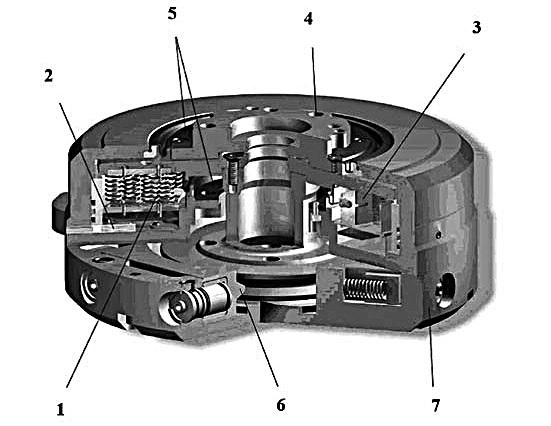
\includegraphics{./img/img11.jpg}	
		\caption{
			\textbf{ Шести компонентный силомоментный датчик FTC-L-50–40 (фирма
				SСHUNK, США):}						
			1 — упругий элемент; 2 — волоконно-оптический
			интерфейс; 3 — фотодиодный преобразователь; 4 —
			узел крепления датчика; 5 — сильфонные уплотнения
			для защиты от пыли; 6 — блокиратор (защита от перегрузок); 7 — алюминиевый корпус
		}     
		\label{fig_img11}
	\end{figure}
	\begin{figure}[ht]
		\centering		 
		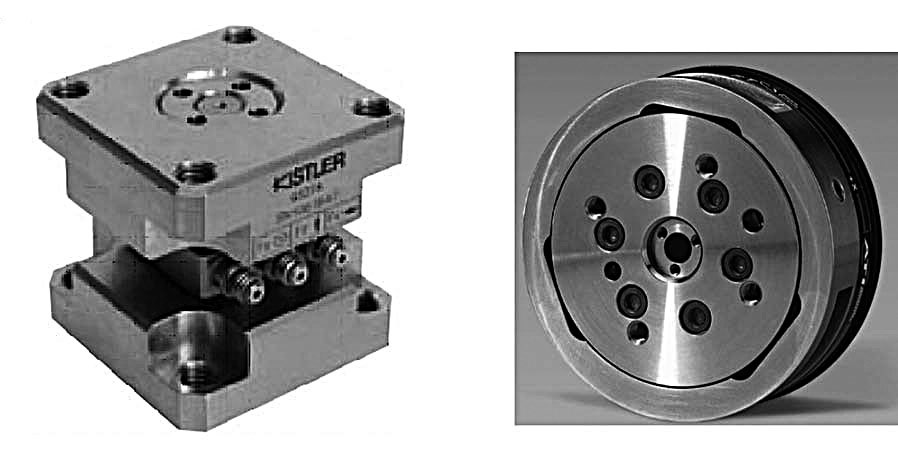
\includegraphics[width=6in]{./img/img12.jpg}	
		\caption{
			\textbf{Силовые датчики на пьезопреобразователях:}			
				a — трех компонентный датчик силы 9328A (фирма Kistler, Германия); б — шести компонентный силомоментный датчик Gamma(фирма ATI, США)
		}     
		\label{fig_img12}
	\end{figure}
	\subsection {Тензорезистивные датчики}
	Тензометрический датчик — датчик, преобразующий величину деформации в удобный для измерения сигнал (обычно электрический), основной компонент тензометра (прибора для измерения деформаций). Существует множество способов измерения деформаций: Среди электронных тензодатчиков, наибольшее распространение получили тензорезистивные датчики.
	
	Тензорезистивный датчик обычно представляет собой специальную упругую конструкцию с закреплённым на ней тензорезистором и другими вспомогательными деталями. После калибровки, по изменению сопротивления тензорезистора можно вычислить степень деформации, которая будет пропорциональна силе, приложенной к конструкции. На Рисунке 1.3 показан пример получивших широкое распространение тензорезистивных датчиков силы.	
	\begin{figure}[ht]
		\centering		 
		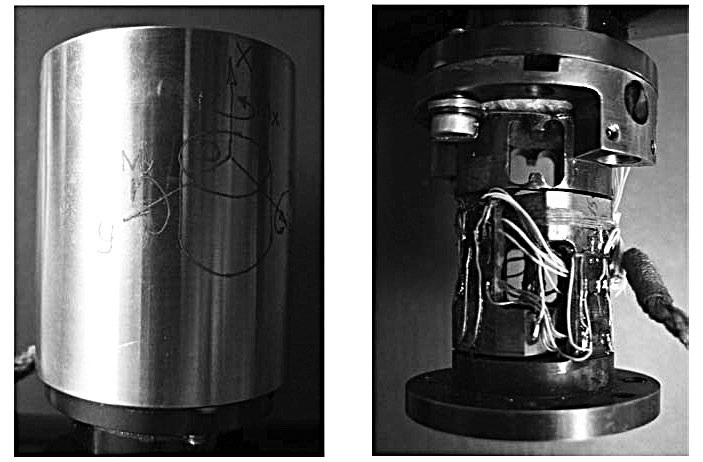
\includegraphics[width=6in]{./img/img13.jpg}	
		\caption{
			\textbf{Шести компонентный силомоментный датчик
				на тензорезисторах СМД (ЦНИИМаш, Россия).}
				Справа — датчик со снятым кожухом
		}     
		\label{fig_img13}
	\end{figure}
	\subsection {Наблюдатели}
	Наряду с устройствами непосредственного определения силы
	существуют так же различные косвенные способы оценки силы с помощью вычислительных устройств, так называемых наблюдателей.
	
	Например, развиваемый электрическим двигателем момент можно
	оценить по величине тока питания. По этим данным с помощью
	математической модели механической системы манипулятора
	может быть рассчитано результирующее усилие в рабочем органе
	манипулятора. Предложены различные алгоритмы и схемы наблюдателей, которые дают оценку этого усилия.
	
	При невысоких требованиях к точности определения усилия
	такие устройства могут быть предпочтительнее датчиков силы, т. к.с 
	они существенно дешевле и проще, не требуют вмешательства
	в конструкцию манипулятора. Наблюдатели могут также применяться в комбинации с силомоментными датчиками.
	Применение наблюдателей силы~--- сравнительно новое направление в робототехнике.
	\section {Обоснование выбора}
	Т.к. мы ставим перед собой задачу обработки моментов и сил, то
	нам подойдёт только тензорезистивный датчик, построенный на кремниевых кристаллах. Наш выбор пал на ATI F/T IP60 Delta в силу качества производства и простоты использования датчика.В качестве робота-манипулятора был выбран Kawasaki fs06n, в качестве контроллера управления - Kawasaki D71.
	\newpage
	\begin{thebibliography}{99}
	\bibitem{yurevich}Юревич, Е. И. Сенсорные системы в робототехнике : учебное пособие / Е. И. Юревич. — СПб. : Изд-во Политехн. ун-та, 2013. — 100 с.	
	\bibitem{vasilenko} Василенко, H.B. Основы робототехники / H.B. Василенко К.Д. Никитин В.П. Пономарёв А.Ю. Смолин — Томск : МГП  РАСКО, 1993 — 474 с.	
	\end{thebibliography}	

\end{document}